\documentclass[10pt]{article}

\def\Type{LessonCaelan}
\def\TypeNum{Lesson 9}
\def\TypeTitle{Properties of Exponential \& Logarithmic Functions }
\def\Semester{Fall 2021} %Not Used 
\def\Course{MATH 1190 \& 1210}
\def\Targets{ {\bf \color{ProcessBlue}F2} }

\usepackage{preambleDJ}

\usepackage{ragged2e}


%%%%%%%%%%%% BEGIN DOCUMENT %%%%%%%%%%%%%%%
%%%%%%%%%%%% BEGIN DOCUMENT %%%%%%%%%%%%%%%
%%%%%%%%%%%% BEGIN DOCUMENT %%%%%%%%%%%%%%%
%%%%%%%%%%%% BEGIN DOCUMENT %%%%%%%%%%%%%%%
%%%%%%%%%%%% BEGIN DOCUMENT %%%%%%%%%%%%%%%



\begin{document}

\pagestyle{otherpages}
\thispagestyle{firstpage}
\vs{.6}

\textbf{Intended Learning Outcomes}
After this lesson, you will be able to 

\begin{itemize}
    \item Apply the properties of exponents and logarithms to simplify an expression. (\target{F2})
    \item Find the values of logarithmic expressions. (\target{F2})
    \item Know properties of exponential and logarithmic function to find their domain, range, and common limits. (\target{F2})
    \item solve equations involving exponential and logarithmic functions. (\target{F2})
\end{itemize}

\vspace{-0.5cm}

\hrulefill


{\bf Properties of Exponents}


\,\hfill
\fbox{$a^x=\underbrace{a\cdot a\cdot a\cdots a}_{x\text{ copies}}$}
\hfill
\fbox{$a^{-x} = \dfrac{1}{a^x}$}
\hfill
\fbox{$a^x a^y = a^{x+y}$}
\hfill
\fbox{$\dfrac{a^x}{a^y}=a^{x-y}$}
\hfill
\fbox{$(a^x)^y = a^{xy}$}
\hfill
\fbox{$a^{x/y}=\sqrt[y]{a^x}$}
\hfill
\,


% when whole numbers, exponents indicate the number of copies of the base being multiplied together -> properties of exponents
\example{\color{ProcessBlue}F2} Simplify the expression below by rewriting exponential expression to contain only positive exponents, expanding exponential expressions (when possible), and using properties of multiplication and division.\\

$\left( \dfrac{ 2^{-3}e^4 }{ 2e^3 } \right)^2$

\vfill

\exercise{\color{ProcessBlue}F2} Simplify each expression below by rewriting exponential expression to contain only positive exponents, expanding exponential expressions, and using properties of multiplication and division.

\begin{enumerate}
\item[(a)] $\sqrt{\dfrac{ e^{7} }{ e^{11} }}$
    \vfill
\item[(b)] $\dfrac{ 2x^{-4}\sqrt{x^{3}} }{ 2^{-5}x^{1/2} }$
    \vfill
\item[(c)] $(a+b)^2$
    \vfill
\end{enumerate}

%%%%%%%%%
\newpage%
%%%%%%%%%


{\bf Properties of Logarithms}


\,\hfill 
\fbox{$\log_a(x)=b$ means $a^b = x$}
\hfill
\fbox{\begin{minipage}{0.15\textwidth}\begin{center}$\log_a(a^x)=x$\\[0.05in] $a^{\log_a(x)}=x$\end{center}\end{minipage}}
\hfill\,\\

\,\hfill
\fbox{$\log_a(x)+\log_a(y)=\log_a(xy)$}
\hfill
\fbox{$\log_a(x)-\log_a(y)=\log_a\left(\dfrac{x}{y}\right)$}
\hfill
\fbox{$p\log_a(x)=\log_a(x^p)$}
\hfill\,

% logarithms indicate the power to which the base must be raised in order to obtain the input -> properties of logarithms

\example{\color{ProcessBlue}F2} / \exercise{\color{ProcessBlue}F2} Evaluate the following:\\

\begin{minipage}[t][2in]{0.47\textwidth}
\begin{enumerate}
\item[(a)] ({\bf\color{blue}Example}) $\log_2\left( 8\right)$
    \vfill

\item[(b)] ({\bf\color{blue}Example}) $\ln\left( \dfrac{1}{\sqrt{e}} \right)$
    \vfill

\end{enumerate}
\end{minipage}
%
\hfill
%
\begin{minipage}[t][2in]{0.5\textwidth}
\begin{enumerate}
\item[(c)] ({\bf\color{blue}Exercise}) $\log_5\left(\sqrt[3]{25}\right)$
    \vfill

\item[(d)] ({\bf\color{blue}Exercise}) $\ln\left( \dfrac{e^5}{e^7}\right)$
    \vfill

\end{enumerate}
\end{minipage}

\example{\color{ProcessBlue}F2} Condense \& simplify the following logarithmic expression completely:\\ 

$\ln(e-1) + \ln(e^2+e) - \ln(e^4-e^2)$

    \vfill
    \vfill
    
\exercise{\color{ProcessBlue}F2} Condense \& simplify the following logarithmic expressions completely:
\begin{enumerate}
\item[(a)] $\log_5 50+\log_5 7-\log_5 14$
    \vfill\vfill
\item[(b)] $\ln(e^2+e)-\ln(e^2-1)+\ln(e^2-e)$\\[0.3in]
    \vfill
    \vfill
%\item[(c)] ({\bf\color{blue}Extra Practice}) $2\log t+3\log (t+1)-\frac13\log(t^3+2t^2+t)$
    %\vfill
    %\vfill
\end{enumerate}

%%%%%%%%%
\newpage%
%%%%%%%%%





{\bf Exponential  Functions}\vs{-.1}\\

The behavior of an exponential function depends upon  the base $a$. Let's experiment and see if we can make a conjecture, i.e. an educated guess, about how the base impacts the graph of an exponential function. Let's start by sketching the graphs of $f(x)=2^x$ and $\ds g(x)=\left(\frac12\right)^x$.

%\setlength{\baselineskip}{12pt}

\exercise{\color{ProcessBlue}F2} Fill in the tables of values below, then sketch the graphs of $f(x)=2^x$ and $\ds g(x)=\left(\frac12\right)^x$. Answer the prompts that follow.\\
\def\sz{0.15in}
\mpageTth{.33}{.33}{.33}{
    \begin{center}
        \begin{tabular}{ c | c }
        $x$ & $f(x)=2^x$\\[0.05in]
        \hline
            & \\[-0.1in]
        $3$ & \\[\sz]
        $2$ & \\[\sz]
        $1$ & \\[\sz]
        $0$ & \\[\sz]
        $-1$ & \\[\sz]
        $-2$ & \\[\sz]
        $-3$ & \\[\sz]
        \end{tabular}
    \end{center}
}{
    \begin{center}
        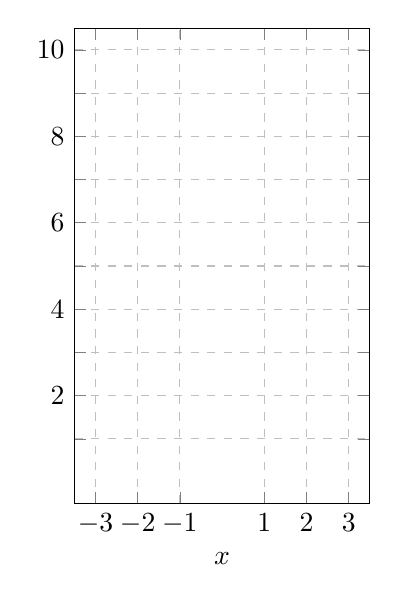
\begin{tikzpicture}
        \begin{axis}[
        xlabel={$x$},
        xtick       = {-3,-2,-1,1,2,3},
        xticklabels = {$-3$,$-2$,$-1$,$1$,$2$,$3$},
        ytick       = {-3,-2,-1,1,2,3,4,5,6,7,8,9,10},
        yticklabels = { ,$-2$, , ,$2$, ,$4$, ,$6$, ,$8$, ,$10$},
        samples     = 320,
        domain      = -3.5:3.5,
        %restrict y to domain=-2.5:4.5,
        xmin = -3.5, xmax = 3.5,
        ymin = -0.5, ymax = 10.5,
        width = 2.1in, height = 3in,
        grid=both, grid style=dashed
        ]
        \end{axis}
        \end{tikzpicture}
    \end{center}
}{
    \begin{center}
        \begin{tabular}{ c | c }
        $x$ & $g(x)=\left(\frac12\right)^x$\\[0.05in]
        \hline
            & \\[-0.1in]
        $3$ & \\[\sz]
        $2$ & \\[\sz]
        $1$ & \\[\sz]
        $0$ & \\[\sz]
        $-1$ & \\[\sz]
        $-2$ & \\[\sz]
        $-3$ & \\[\sz]
        \end{tabular}
    \end{center}
}
\vs{-.1}~\\
{\bf  \blue{Conjecture/ Educated Guessing }} Consider our sketching exercise and make an educated guess about the behavior of $f(x)=a^x$. \vs{-.1}\\
%\tasksA{2}{
%\task  When $f(x)=a^x$ and  base $\mathbf{a>1}$, does the graph appear to increase to infinity or decrease to $0$ as $x$ gets larger? \label{eqn1}
%\task  When $f(x)=a^x$ and  base $\mathbf{a>1}$, how would you describe the  behavior of the slope of tangent lines as $x$ gets larger?\vs{1}
%\task When $f(x)=a^x$ and  base $\mathbf{0<a<1}$, does the graph appear to increase to infinity or decrease to $0$ as $x$ gets larger?\label{eqn2}
%\task When $f(x)=a^x$ and  base $\mathbf{0<a<1}$, how would you describe the  behavior of the slope of tangent lines as $x$ gets larger?
%}
%\newpage
\mpageT{.45}{.45}[\hs{.35}]{
\enumA{
\item When $f(x)=a^x$ and  base $\mathbf{a>1}$, does the graph appear to increase to infinity or decrease to $0$ as $x$ gets larger? \label{eqn1}
\vs{.75}
\item When $f(x)=a^x$ and  base $\mathbf{0<a<1}$, does the graph appear to increase to infinity or decrease to $0$ as $x$ gets larger?\label{eqn2}
}
}{
 {\em Conjecture} Based on your response in \ref{eqn1} and \ref{eqn2} what are some reasonable things you might say about each of the following symbols? Consider how the words above might translate to mathematical statements.\\\\
  \renewcommand{\arraystretch}{2.5} 
  %\rowcolor{darkgray}
 \begin{tabularx}{1.3\textwidth}{| L{.3} L{.25} | L{.3} L{.25} |}     \hline
%\multicolumn{1}{c}{$a>1$} & \multicolumn{1}{x}{$0<a<1$}\\
\multicolumn{2}{ |C{.5} | }{$\mathbf{a>1}$ }&  \multicolumn{2}{ C{.5} | }{ $\mathbf{0<a<1}$} \\ \hline
$\bullet$   $f^{\prime}(x)$  &\unline{.5}{}{.25} & $\bullet$   $f^{\prime}(x)$ & \unline{.5}{}{.25} \\
$\bullet$   $\ds \lim_{x\to \infty}a^x=$  & \unline{.5}{}{.25}  & $\bullet$ $\ds \lim_{x\to \infty}a^x=$  & \unline{.5}{}{.25}\\
$\bullet$   $\ds \lim_{x\to -\infty}a^x=$ &  \unline{.5}{}{.25}  & $\bullet$ $\ds \lim_{x\to -\infty}a^x=$  & \unline{.5}{}{.25} \vs{.2}\\  \hline
%& &&\\ \hline
\end{tabularx}
  \renewcommand{\arraystretch}{1} 
}
~\\\\
%\setlength{\baselineskip}{18pt}
\mpageT{.45}{.45}[\hs{.35}]{
{\bf \blue{Exponential Functions}} 
\itemI{
\item $y=f(x)=a^x$\\
\item Domain (i.e. inputs):\\
\item Range (i.e. outputs):\\
}
}{
{\bf \blue{Power Functions}}
\itemI{
\item $y=f(x)=x^a$\\
\item Domain (i.e. inputs):\\
\item Range (i.e. outputs):\\
}
}
\vs{.3}\\
\newpage
{\bf Logarithmic functions}

The behavior of a logarithmic function $\ds \log_a(x)$  depends upon  the base $a$. Let's experiment and see if we can make a conjecture, i.e. an educated guess, about how the base impacts the graph of an exponential function. Let's start by sketching the graph of $f(x)=\log_2(x)$.

%\item {\em Conjecture} Based on your response in \ref{eqn1} and \ref{eqn2} what are some reasonable things you might say about each of the following symbols? Consider how the words above might translate to mathematical statements.
\exercise{\bf\color{ProcessBlue}F2} Fill in the table of values below, then sketch the graph of $f(x)=\log_2(x)$. Answer the prompts that follow.

\mpageT{.33}{.67}{
    \begin{center}
        \begin{tabular}{ c | c }
        $x$ & $f(x)=\log_2(x)$\\[0.05in]
        \hline
            & \\[-0.1in]
        $1/8$ & \\[\sz]
        $1/4$ & \\[\sz]
        $1/2$ & \\[\sz]
        $1$ & \\[\sz]
        $2$ & \\[\sz]
        $4$ & \\[\sz]
        $8$ & \\[\sz]
        \end{tabular}
    \end{center}
}{
    \begin{center}
        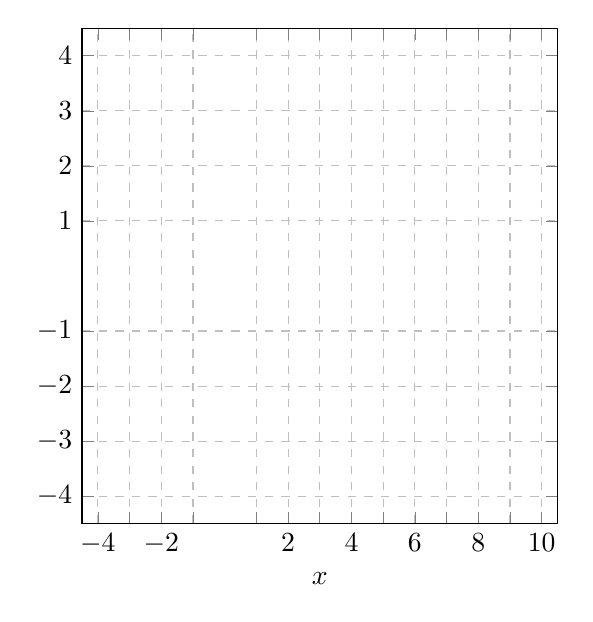
\begin{tikzpicture}
        \begin{axis}[
        xlabel={$x$},
        ytick       = {-4,-3,-2,-1,1,2,3,4},
        yticklabels = {$-4$,$-3$,$-2$,$-1$,$1$,$2$,$3$,$4$},
        xtick       = {-4,-3,-2,-1,1,2,3,4,5,6,7,8,9,10},
        xticklabels = { $-4$,,$-2$, , ,$2$, ,$4$, ,$6$, ,$8$, ,$10$},
        samples     = 320,
        domain      = -4.5:4.5,
        %restrict y to domain=-2.5:4.5,
        xmin = -4.5, xmax = 10.5,
        ymin = -4.5, ymax = 4.5,
        width = 3in, height = 3.1in,
        grid=both, grid style=dashed
        ]
        \end{axis}
        \end{tikzpicture}
    \end{center}
}
\vs{.2}~\\
{\bf  \blue{Conjecture/ Educated Guessing }} Consider our sketching exercise and make an educated guess about the behavior of $f(x)=\log_a (x)$. \\
\vs{-.3}
\mpageT{.45}{.45}[\hs{.35}]{
\enumA{
\item When $f(x)=\log_a(x)$ and  base $\mathbf{a>1}$, does the graph appear to increase to infinity, increase to negative infinity or decrease to $0$ as $x$ gets larger? \label{eqn3}
\vs{.75}
\item As $x$ gets closer to $0$, does the graph appear to increase to infinity, increase to negative infinity or decrease to $0$?\label{eqn4}
}
}{
 {\em Conjecture} Based on your response in \ref{eqn3} and \ref{eqn4} what are some reasonable things you might say about each of the following symbols? Consider how the words above might translate to mathematical statements.\\\\
  \renewcommand{\arraystretch}{2.5} 
 \begin{tabularx}{1.2\textwidth}{| L{.4} L{.25} | L{.25} L{.2} |}     \hline
\multicolumn{4}{ |C{1} | }{$\qquad \qquad \mathbf{f(x)=\log_a(x),\qquad a>1}$}  \\ \hline
$\bullet$   $f^{\prime}(x)$  &\unline{.5}{}{.25} & $\bullet$   $\log_a(0)$ & \unline{.5}{}{.25} \\
$\bullet$   $\ds \lim_{x\to \infty} \log_a(x)=$  & \unline{.5}{}{.25}  & $\bullet$ $\ds \log_a(-3)$  & \unline{.5}{}{.25}\\
$\bullet$   $\ds \lim_{x\to 0^+} \log_a(x)=$ &  \unline{.5}{}{.25}   &    & \vs{.2}\\ \hline
%%& &&\\ \hline
\end{tabularx}
  \renewcommand{\arraystretch}{1} 
}
\vs{.25}\\
{\bf \blue{Logarithmic functions}}
\tasksI{3}{
\task $y=f(x)=\log_a(x)$\\\\
\task Domain (i.e. inputs):\\\\
\task Range (i.e. outputs):\\
}
\vs{.25}~\\
{\em Key Idea: Inverse} 

\newpage


\example{\color{ProcessBlue}F2} Solve the following equations for $x$.
%
\enumA{
\item $2^x=10$\vfill
\item $2^{4+2/x} = 8$

    \vfill

\item $\log_3(x+4)+\log_3(x-2)=3$

    \vfill
    \vfill

}
\newpage
The following problem appeared on an assessment during the Fall 2023 semester.\\

{\bf\color{blue}Exam Practice 1.} \reversemarginpar \marginnote{\fbox{\bf\color{ProcessBlue}F2}}
%
Respond to the following prompts.
\begin{enumerate}
    
        \item[(a)] Evaluate: \quad $\displaystyle \log_{2} \left( \frac{1}{32} \right)=$\rule[-8pt]{1in}{0.4pt}
        
        
        \item[(b)] Simplify the expression completely: \quad $\displaystyle e^{3 \ln( 5)} - \ln( e ) + \frac{\ln( e^3)}{\ln( e^5)} - \ln( e^3 e^5) $
        
        
        \vfill
    
        \item[(c)] Solve the following equation for $x$: \quad $\displaystyle \log_2(x - 3) + \log_2(x + 1) = 5$
 
        \vfill
        \vfill
       
    \end{enumerate}


%%%%%%%%%
\newpage%
%%%%%%%%%

{\bf\color{blue}Extra Practice 1.} \reversemarginpar \marginnote{\fbox{\bf\color{ProcessBlue}F2}}
%
Find all possible solutions to the following equations.
\begin{enumerate}
\item[(a)] $5^x-4=0$
    \vfill
\item[(b)] $5^x+5=0$
    \vfill
\item[(c)] $5^{2x}+5^x-20=0$
    \vfill
\item[(d)] $2e^{2x}-5e^x+2=0$
    \vfill
    \vfill
\end{enumerate}

\newpage
{\bf\color{blue}Extra Practice 2.} \reversemarginpar \marginnote{\fbox{\bf\color{ProcessBlue}F2}} 
%
Find all possible solutions to the following equations.
\begin{enumerate}
\item[(a)] $\log_5(x+2)-2=0$
\vfill

\item[(b)] $5^{x+2}-2=0$
\vfill
\item[(c)] $\log_5(x+2)-2 = \log_5(x)$
\vfill
\item[(d)] $5^{x+2}-2=5^{x}$
\vfill
\end{enumerate}

\end{document}
